\documentclass[2pt, a4paper, fleqn]{extarticle}

\usepackage[T2A]{fontenc}
\usepackage[utf8]{inputenc}
\usepackage[english,russian]{babel}
\usepackage{url}
%\usepackage{pscyr}

%\renewcommand{\rmdefault}{ftm}
\usepackage{setspace}
\onehalfspacing

\usepackage{changepage}
\usepackage{indentfirst} %первый абзац
%%\usepackage{moreverb}
\usepackage[noend]{algorithmic}
\usepackage{amssymb, amsmath, multicol,amsthm}
%%
\usepackage{enumitem, multicol}
\usepackage{titleps,lipsum}
%%
\usepackage{mathrsfs}
\usepackage{verbatim}
\usepackage{pb-diagram}
\usepackage{graphicx}
\graphicspath{ {images/} }
\usepackage{wrapfig}
\usepackage{xcolor}
\definecolor{new}{RGB}{255,184,92}
\definecolor{news}{RGB}{112,112,112}
\usepackage{wallpaper}
\usepackage{float}
\usepackage{hyperref}
\hypersetup{
%colorlinks=true,%
%linkcolor=news,%
linkbordercolor=new,
}



\usepackage{geometry}
\geometry{top=1cm,bottom=2cm,left=1cm,right=1cm}

%\flushbottom
%\ruggedbottom

\binoppenalty=5000
\parindent=0pt

\newcommand{\EDS}{\ensuremath{\mathscr{E}}}
\newcommand*{\hm}[1]{#1\nobreak\discretionary{}%
{\hbox{$\mathsurround=0pt #1$}}{}}
\newcommand{\divisible}{\mathop{\raisebox{-2pt}{\vdots}}}
\renewcommand{\theequation}{\arabic{equation}}
\def\hm#1{#1\nobreak\discretionary{}{\hbox{$#1$}}{}}
\newcommand{\bbskip}{\bigskip \bigskip}



%%\DeclareMathOperator{\tg}{tg}
%%\DeclareMathOperator{\ctg}{ctg}

\let\leq\leqslant
\let\geq\geqslant



% Remove brackets from numbering in List of References
\makeatletter
\renewcommand{\@biblabel}[1]{\quad#1.}
\makeatother

\begin{document}

Уравнение, решаемое на втором шаге расщепления:

$$\dfrac{\partial n}{\partial t} = \dfrac{1}{a\cos\varphi} \dfrac{\partial }{\partial \varphi}\left[\dfrac{D}{a}\cdot(\cos^2  I \cos\varphi)\cdot\dfrac{\partial n}{\partial \varphi}-D\cdot(\sin I\cos I\cos\varphi)\cdot \dfrac{\partial n}{\partial z} - u\cdot(\sin I \cos I \cos\varphi)\cdot n \right]$$

Здесь $u = D\left(\dfrac{1}{T_p}\dfrac{\partial T_p}{\partial z}+\dfrac{1}{H}\right)$~---~эффективная скорость из первого шага, $I = \arctg(2\tg \varphi)$.

На первом этапе решаем задачу без смешанной производной. В качестве начальных условий выступает решение уравнения с первого шага расщепления. Введём функции $A(\varphi) = \cos \varphi \cdot \cos^2(\arctg(2\tg \varphi))$ и $B(\varphi) = \cos\varphi \cdot \sin(2\arctg(2\tg \varphi))$.

С помощью этих функций задачу можно переписать в следующем виде: 
$$\dfrac{\partial n}{\partial t} = \dfrac{1}{\cos\varphi} \dfrac{\partial }{\partial \varphi}\left[\dfrac{D}{a^2}A(\varphi)\dfrac{\partial n}{\partial \varphi}-\dfrac{D}{2a}B(\varphi) \dfrac{\partial n}{\partial z} - \dfrac{u}{2a}B(\varphi) n \right]$$
Исследуем асимптотическое поведение слагаемых вблизи полюсов (при $\varphi = \pm\dfrac{\pi}{2}$).

Графики функций $A$ и $B$ приведены ниже: 

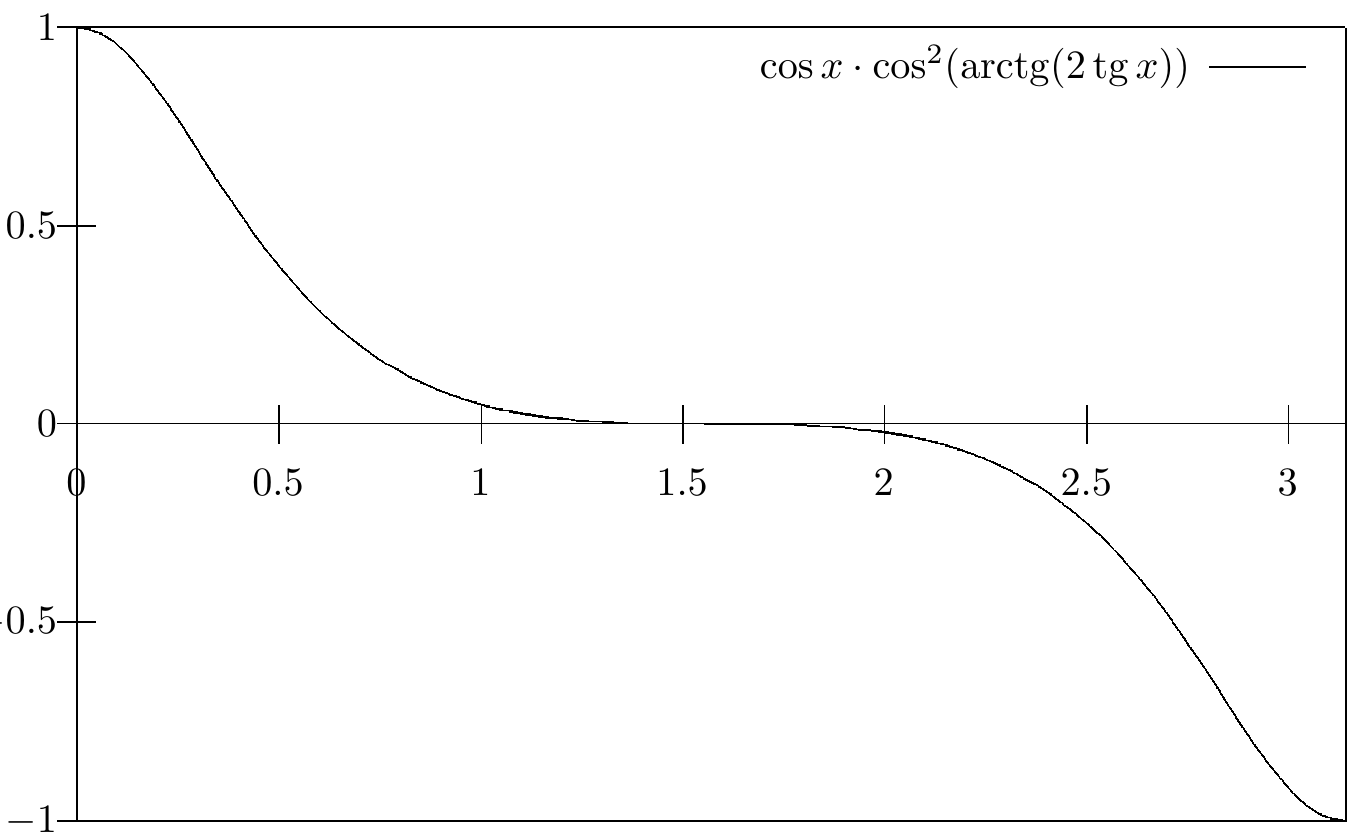
\includegraphics[scale=0.25]{A}

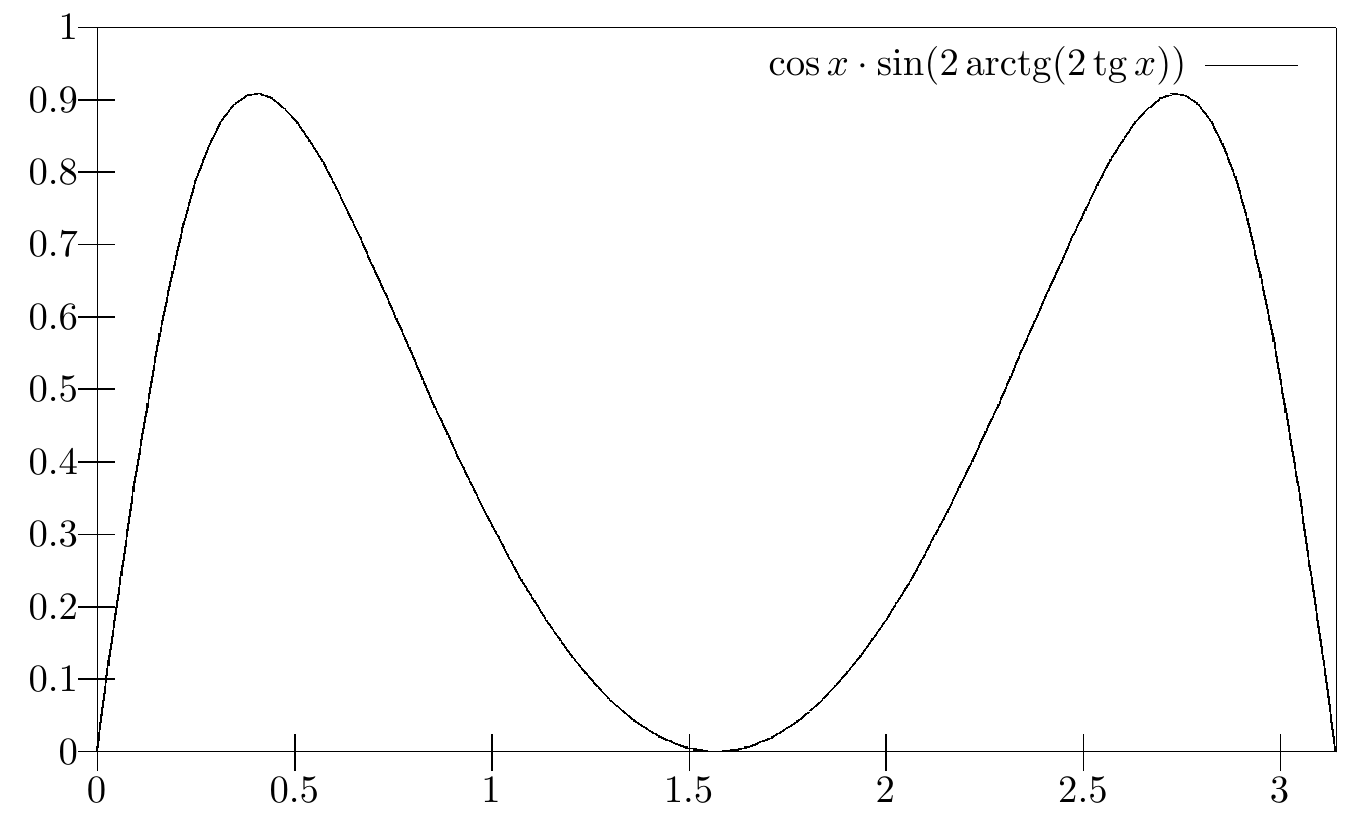
\includegraphics[scale=0.25]{B}

Обе функции в точке $\varphi = \dfrac{\pi}{2}$ касаются оси абсцисс~---~имеют нули по крайней мере второго порядка, поэтому особенность в уравнении устранимая.

Имеют место следующие разложения при $\varphi\rightarrow\dfrac{\pi}{2}$: $$A(\varphi)=-\dfrac{1}{4}\cdot\left(\varphi-\dfrac{\pi}{2}\right)^3-\dfrac{1}{16}\cdot\left(\varphi-\dfrac{\pi}{2}\right)^5+o\left(\left(\varphi-\dfrac{\pi}{2}\right)^6\right)$$ $$B(\varphi) = 1\cdot\left(\varphi-\dfrac{\pi}{2}\right)^2-\dfrac{1}{12}\cdot \left(\varphi-\dfrac{\pi}{2}\right)^4+o\left(\left(\varphi-\dfrac{\pi}{2}\right)^5\right)$$

Соответственно, при $x\rightarrow-\dfrac{\pi}{2}$: $$A(\varphi)=\dfrac{1}{4}\cdot\left(\varphi+\dfrac{\pi}{2}\right)^3+\dfrac{1}{16}\cdot\left(\varphi+\dfrac{\pi}{2}\right)^5+o\left(\left(\varphi+\dfrac{\pi}{2}\right)^6\right)$$ $$B(\varphi) = -1\cdot\left(\varphi+\dfrac{\pi}{2}\right)^2+\dfrac{1}{12}\cdot \left(\varphi+\dfrac{\pi}{2}\right)^4+o\left(\left(\varphi+\dfrac{\pi}{2}\right)^5\right)$$



Обозначим $\varphi-\dfrac{\pi}{2} = x$. При $x\rightarrow 0$ заметим, что: $$\dfrac{1}{\cos\varphi}\dfrac{\partial}{\partial\varphi}\left(A(\varphi)\dfrac{\partial n}{\partial\varphi}\right) = \dfrac{1}{\cos\varphi}\dfrac{\partial A}{\partial\varphi}\dfrac{\partial n}{\partial\varphi} + \dfrac{A}{\cos\varphi}\dfrac{\partial^2 n}{\partial\varphi^2} \approx \dfrac{1}{x-\frac{x^3}{6}}\left(-\dfrac14\cdot 2x^2\right)\dfrac{\partial n}{\partial\varphi} - \dfrac14\dfrac{x^2}{1-\frac{x^2}{6}}\dfrac{\partial^2 n}{\partial\varphi^2}\approx$$ $$\approx -\dfrac12x\dfrac{\partial n}{\partial\varphi}-\dfrac14x^2\dfrac{\partial^2 n}{\partial\varphi^2}=-\dfrac12\left(\varphi-\dfrac{\pi}{2}\right)\dfrac{\partial n}{\partial\varphi}-\dfrac14\left(\varphi-\dfrac{\pi}{2}\right)^2\dfrac{\partial^2 n}{\partial\varphi^2}$$

$$\dfrac{1}{\cos\varphi}\dfrac{\partial}{\partial\varphi}\left(B(\varphi)\dfrac{\partial n}{\partial z}\right) = \dfrac{1}{\cos\varphi}\dfrac{\partial B}{\partial\varphi}\dfrac{\partial n}{\partial z} + \dfrac{1}{\cos\varphi}B\dfrac{\partial^2 n}{\partial \varphi\partial z} \approx 2\dfrac{\partial n}{\partial z}+\left(\varphi-\dfrac{\pi}{2}\right)\dfrac{\partial^2 n}{\partial \varphi\partial z}$$

$$\dfrac{1}{\cos\varphi}\dfrac{\partial}{\partial\varphi}\left(B(\varphi)n\right) = \dfrac{1}{\cos\varphi}\dfrac{\partial B}{\partial\varphi}n + \dfrac{1}{\cos\varphi}B\dfrac{\partial n}{\partial \varphi} \approx 2n+\left(\varphi-\dfrac{\pi}{2}\right)\dfrac{\partial n}{\partial \varphi}$$

Для полного уравнения используем следующую схему:
$$\dfrac{n_{i,j}^{t+1}-n_{i,j}^t}{\tau} = \dfrac{1}{\cos\varphi_j} \bigg[\dfrac{D}{a^2}\left(A(\varphi_{j+1/2})\dfrac{n_{i, j+1}^{t+1}-n_{i,j}^{t+1}}{\Delta\varphi^2}-A(\varphi_{j-1/2})\dfrac{n_{i,j}^{t+1}-n_{i,j-1}^{t+1}}{\Delta\varphi^2}\right)-\dfrac{u}{2a}\left(\dfrac{B(\varphi_{j+1})n_{i,j+1}^{t+1}-B(\varphi_{j-1})n_{i,j-1}^{t+1}}{2\Delta\varphi}\right) -$$ $$- \dfrac{D}{2a}\left(\dfrac{|u_z|+u_z}{2}\dfrac{n_{i,j+1}^{t+1}-n_{i,j}^{t+1}}{\Delta\varphi}+\dfrac{|u_z|-u_z}{2}\dfrac{n_{i,j}^{t+1}-n_{i,j-1}^{t+1}}{\Delta\varphi}\right) \bigg]$$

(Консервативность?..)

Здесь введено обозначение $u_z = \dfrac{1}{n}\dfrac{\partial n}{\partial z} = \dfrac{\partial \ln n}{\partial z}$. При этом значения $n$ для вычисления $u_z$ берутся с предыдущего временного шага.

При $j = 1$ $(\varphi = -90^\circ)$ и $j = N_\varphi$ $(\varphi = +90^\circ)$ используем граничные условия Дирихле~---~равенство распределения на полюсах дневному распределению одномерной задаче в $z$-проекции без учета широтной зависимости.

При $i = 1$ $(z = 100\mbox{ } \mbox{км})$ также ставим граничное условие Дирихле~---~на нижней границе по $z$ решение совпадает с $P/k$, полученным на первом шаге.

На верхней границе требуется граничное условие для определения $u_z$.

Поток на границе $z=z_{ub}$: $$\dfrac{D}{a^2}A(\varphi_{j+1/2})\dfrac{n_{N, j+1}-n_{N, j}}{h}-\dfrac{u}{2a}\dfrac{B(\varphi_{j+1})n_{N, j+1}+B(\varphi_j)n_{N, j}}{2\Delta\varphi}-\dfrac{D}{2a}\left(\dfrac{|u_z|}{2}\dfrac{n_{N, j+1}+n_{N, j}}{\Delta\varphi}+\dfrac{u_z}{2}\dfrac{n_{N, j+1}-n_{N, j}}{\Delta\varphi}\right) = F_{y}$$



\end{document}



